\documentclass[11pt,oneside]{book}

\usepackage[a4paper,margin=1in]{geometry}
\usepackage[T1]{fontenc}
\usepackage[utf8]{inputenc}
\IfFileExists{newtxtext.sty}{
  \usepackage{newtxtext,newtxmath}
}{
  \usepackage{mathptmx}
}
\usepackage{microtype}
\usepackage{setspace}
\usepackage{graphicx}
\usepackage{xcolor}
\definecolor{lightblue}{rgb}{0.68,0.85,0.90}
\definecolor{lightgreen}{rgb}{0.56,0.93,0.56}
\definecolor{lightgray}{rgb}{0.83,0.83,0.83}
\usepackage{booktabs}
\usepackage{longtable}
\usepackage{array}
\usepackage{tabularx}
\usepackage{caption}
\usepackage{subcaption}
\usepackage{listings}
\usepackage{hyperref}
\usepackage{tocloft}
\usepackage{fancyhdr}
\usepackage{enumitem}
\usepackage{titlesec}
\usepackage{float}
\usepackage{tikz}
\usepackage{verbatim}
\usepackage{amsmath}
\usepackage{amssymb}
\usepackage{url}

\hypersetup{
  colorlinks=true,
  linkcolor=black,
  urlcolor=blue,
  citecolor=black,
  pdftitle={WhisperTunnel VPN: Architecture, Implementation, and Evaluation},
  pdfauthor={Project Technical Report},
  pdfsubject={Educational VPN System Analysis}
}

\setstretch{1.05}
\setlength{\parskip}{0.25em}
\setlength{\parindent}{1.2em}
\setlength{\headheight}{14pt}

\pagestyle{fancy}
\fancyhf{}
\fancyhead[LE,RO]{WhisperTunnel VPN Report}
\fancyhead[RE,LO]{\leftmark}
\fancyfoot[C]{\thepage}

\titleformat{\chapter}[display]
  {\normalfont\bfseries\Large}
  {\chaptertitlename\ \thechapter}{0.5em}{\Huge}

\lstdefinestyle{vpnpython}{
  language=Python,
  basicstyle=\ttfamily\small,
  keywordstyle=\color{blue!60!black}\bfseries,
  commentstyle=\color{green!40!black},
  stringstyle=\color{red!50!black},
  numbers=left,
  numberstyle=\tiny\color{gray},
  stepnumber=1,
  numbersep=8pt,
  showstringspaces=false,
  breaklines=true,
  frame=single,
  rulecolor=\color{black!20}
}

\lstdefinestyle{vpnbash}{
  language=bash,
  basicstyle=\ttfamily\small,
  keywordstyle=\color{blue!60!black}\bfseries,
  commentstyle=\color{green!40!black},
  numbers=left,
  numberstyle=\tiny\color{gray},
  stepnumber=1,
  numbersep=8pt,
  showstringspaces=false,
  breaklines=true,
  frame=single,
  rulecolor=\color{black!20}
}

\newcommand{\imgplaceholder}[2]{
\begin{figure}[H]
  \centering
  \fbox{\begin{minipage}[c][0.25\textheight][c]{0.85\textwidth}
    \centering
    \textbf{Image Placeholder}\\[0.5em]
    #2
  \end{minipage}}
  \caption{#1}
\end{figure}
}

\begin{document}

\frontmatter

\begin{titlepage}
\centering
{\Huge \textbf{WhisperTunnel VPN}\\[0.5em]}
{\LARGE Architecture, Implementation, and Operations Report\\[1.5em]}
{\large Technical Documentation\\}
\vfill
{\large Prepared for the WhisperTunnel Project\\[0.4em]}

{\large Team Members\\[0.3em]}
\begin{tabular}{c}
\large Shudarsan Regmi (CH.SC.U4CYS23055)
\end{tabular}

\vspace{0.6em}
{\large Date: 29 March 2026\\}
\vfill
\begin{minipage}{0.85\textwidth}
\centering
\textit{This report presents a focused engineering analysis of the WhisperTunnel educational VPN implementation. It consolidates architecture, protocol flow, cryptographic design, network setup, implementation walkthroughs, operations guidance, and roadmap recommendations in a publication-style format suitable for academic or technical submission.}
\end{minipage}
\end{titlepage}

\chapter*{Abstract}
WhisperTunnel is a minimal educational Virtual Private Network (VPN) implementation in Python that demonstrates encrypted packet tunneling through Linux TUN interfaces, authenticated transport over TCP, and isolation-oriented validation using network namespaces. This report studies the full codebase and associated scripts, then synthesizes a professional, book-style technical narrative around the system's design and behavior.

The implementation combines AES-GCM payload encryption, a framed packet protocol using length-prefix messages, and a lightweight HMAC-based authentication handshake. It targets conceptual clarity and demonstrability rather than production-hardening. Through direct inspection of modules in \texttt{client/}, \texttt{server/}, \texttt{common/}, and \texttt{scripts/}, this report reconstructs control paths, data paths, component responsibilities, and deployment assumptions.

Beyond architecture exposition, this book includes structured tables, sequence explanations, code listings, operational runbooks, and migration recommendations for evolving the MVP. Image placeholders are inserted throughout to support later inclusion of screenshots, packet captures, topology diagrams, and codebase snapshots.

\chapter*{How to Read This Report}
Readers can approach this document in one of three ways:
\begin{itemize}[leftmargin=2em]
\item \textbf{Fast orientation}: read Chapters 1, 3, and 8.
\item \textbf{Engineering deep dive}: read Chapters 4 through 6 in order.
\item \textbf{Operations focus}: read Chapter 7.
\end{itemize}

\tableofcontents
\listoffigures
\listoftables
\clearpage

\mainmatter

\chapter{Introduction}

\section{Motivation}
Virtual Private Networks are often taught at a conceptual level, while implementation details are hidden inside mature systems such as WireGuard, OpenVPN, and IPSec stacks. WhisperTunnel addresses this educational gap by offering a compact, inspectable codebase that exposes the operational core of a VPN tunnel: packet capture from a virtual interface, cryptographic encapsulation, framed transport, authenticated delivery, and reinjection into a target network stack.

The project is intentionally minimal and Linux-centric. It avoids protocol complexity that would obscure first-principles understanding, while still covering enough subsystems to be meaningful for systems programming, cryptography integration, and network operations training.

\section{Scope of This Report}
This document is a code-driven study of the WhisperTunnel repository. It does not merely restate generic VPN knowledge. Instead, it maps directly to implemented modules and scripts, including:

\begin{itemize}[leftmargin=2em]
\item Python modules under \texttt{custom\_vpn/common}, \texttt{custom\_vpn/client}, and \texttt{custom\_vpn/server}.
\item Runtime orchestration and environment scripts under \texttt{custom\_vpn/scripts}.
\item Validation assets under \texttt{custom\_vpn/tests}.
\item Design narratives in \texttt{README.md} and \texttt{docs/design.md}.
\end{itemize}

\section{Project Objectives Interpreted from Code}
From implementation behavior and accompanying scripts, the practical objectives are:

\begin{enumerate}[leftmargin=2em]
\item Establish an encrypted L3 tunnel between one client and one server.
\item Run clean demonstrations in isolated network namespaces.
\item Maintain readable code pathways for educational use.
\item Provide reproducible setup scripts and baseline diagnostics.
\item Expose known limitations explicitly for pedagogical honesty.
\end{enumerate}

\section{Operational Summary}
At runtime, a client process and server process each attach to a Linux TUN interface. Raw IP packets are read from the local TUN, encrypted with AES-GCM, and framed for transport over a persistent TCP socket. The peer receives framed ciphertext, decrypts it, then writes plaintext packets into its local TUN device. Authentication is performed once at connection setup using timestamped HMAC tokens.

\begin{table}[H]
\centering
\caption{WhisperTunnel at a Glance}
\begin{tabular}{p{0.28\textwidth}p{0.58\textwidth}}
\toprule
\textbf{Dimension} & \textbf{Current Implementation} \\
\midrule
Tunnel type & L3 packet forwarding via Linux TUN \\
Payload protection & AES-256-GCM, random nonce per packet \\
Transport & TCP with 4-byte big-endian length prefix \\
Authentication & Shared-key HMAC token + timestamp validation \\
Concurrency model & Threaded loops (bidirectional forwarding) \\
Client scale & Single client (MVP) \\
Primary test model & Linux network namespaces + pytest \\
\bottomrule
\end{tabular}
\end{table}

\section{Why a Book-Style Report}
A book format is appropriate because this project spans multiple engineering layers:

\begin{itemize}[leftmargin=2em]
\item Application lifecycle and process orchestration.
\item Cryptographic API usage and threat boundaries.
\item Packet protocol mechanics over stream transport.
\item Linux networking internals (TUN, namespaces, NAT, routing).
\item Testability and operational runbooks.
\end{itemize}

These layers are easier to digest in chaptered form with stable references, tables, and figure anchors than in a short project memo.

\section{Reading Outcomes}
After reading this report, a technical reader should be able to:

\begin{enumerate}[leftmargin=2em]
\item Explain how WhisperTunnel moves packets from one namespace to another.
\item Reproduce a local deployment using provided scripts and commands.
\item Evaluate security strengths versus missing controls.
\item Identify bottlenecks and practical paths toward production hardening.
\item Extend the implementation while preserving conceptual clarity.
\end{enumerate}

\section{Method Used for Analysis}
This report is built from static inspection of source files and scripts, complemented by consistency checks between implementation and documentation. No claims are made that exceed visible repository evidence. Where ambiguity exists, the text marks assumptions and proposes verification actions.

\section{Limitations of This Study}
The analysis reflects repository state as of 29 March 2026. Runtime measurements are discussed conceptually unless explicit benchmark outputs are present in code or scripts. Also, script behavior can vary by Linux distribution, iptables backend, and local network policy.

\section{Chapter Roadmap}
Chapter 2 provides background context and concepts. Chapter 3 maps repository structure and responsibilities. Chapters 4 to 6 detail architecture and implementation flow. Chapter 7 focuses on deployment and operations. Chapter 8 concludes with prioritized roadmap guidance.

\chapter{Background and Conceptual Foundations}

\section{VPN Fundamentals Relevant to WhisperTunnel}
A VPN creates a protected path between endpoints by encapsulating original network packets and transmitting them through an intermediate network. In WhisperTunnel, encapsulation occurs in user space: plaintext IP packets read from a TUN interface are encrypted and then sent over TCP.

The tunnel endpoint relationship is symmetric at the data plane:
\begin{itemize}[leftmargin=2em]
\item Endpoint A reads from \texttt{tun0}, encrypts, frames, and sends.
\item Endpoint B receives, deframes, decrypts, and writes to \texttt{tun0}.
\item The reverse direction follows the same sequence concurrently.
\end{itemize}

\section{TUN Interfaces in Linux}
A TUN interface is a virtual point-to-point network interface that operates at layer 3. Programs interact with it through a file descriptor and exchange raw IP packets. This mechanism allows user-space VPN implementations to participate directly in packet forwarding without requiring kernel-space VPN code.

Key implications for WhisperTunnel:
\begin{itemize}[leftmargin=2em]
\item The kernel routes traffic into \texttt{tun0} based on routing tables.
\item User-space reads packets using \texttt{os.read} and writes using \texttt{os.write}.
\item Correct interface setup (IP, MTU, link state) is mandatory for traffic flow.
\end{itemize}

\section{AEAD and AES-GCM}
WhisperTunnel uses AES-GCM, an AEAD (Authenticated Encryption with Associated Data) mode. AEAD provides confidentiality and integrity in one operation. In this implementation:
\begin{itemize}[leftmargin=2em]
\item Key size is 32 bytes (AES-256).
\item Nonce size is 12 bytes (GCM standard size).
\item Nonce is generated per packet via \texttt{os.urandom}.
\item Output format is \texttt{nonce || ciphertext+tag}.
\end{itemize}

The absence of additional authenticated data (AAD) keeps API usage simple for teaching, although AAD could later bind metadata (sequence IDs, protocol version) for stronger contextual validation.

\section{Stream Transport Framing}
TCP is byte-stream oriented and does not preserve application message boundaries. WhisperTunnel solves this by prepending each encrypted payload with a 4-byte big-endian length field.

Mathematically, if $C$ is encrypted payload bytes and $|C|$ is its length, wire format is:
\[
M = \text{uint32\_be}(|C|) \; || \; C
\]

Receiver logic reads exactly 4 bytes first, decodes length, validates against \texttt{MAX\_PACKET\_SIZE}, then reads exactly that many bytes.

\section{Authentication Model}
Connection setup uses a simple shared-key HMAC token:
\begin{itemize}[leftmargin=2em]
\item Token payload includes an 8-byte timestamp.
\item HMAC-SHA256 over timestamp is appended.
\item Peer verifies MAC validity and timestamp age (default 300 s).
\item Server sends acknowledgment token after successful verification.
\end{itemize}

This mechanism provides basic shared-secret proof-of-knowledge but does not provide identity hierarchy, certificate management, or forward secrecy.

\section{Network Namespaces for Test Isolation}
Linux network namespaces create independent network stacks, allowing realistic client/server experiments on one host. WhisperTunnel scripts use namespaces to emulate separate machines while preserving reproducibility.

Benefits include:
\begin{itemize}[leftmargin=2em]
\item Isolated interfaces and routes per namespace.
\item Deterministic topology using veth pairs.
\item Safe teardown and reset with cleanup scripts.
\end{itemize}

\begin{figure}[H]
\centering
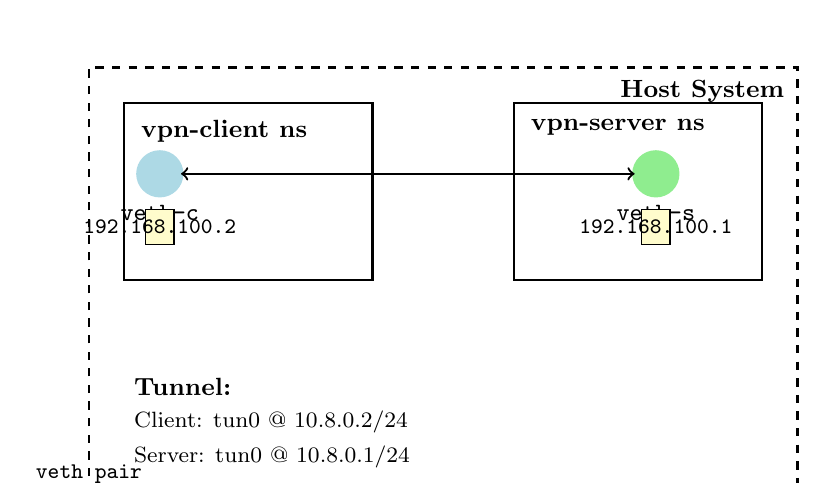
\begin{tikzpicture}[scale=0.9, every node/.style={font=\small}]
  % Host system box
  \draw[thick, dashed] (0,0) rectangle (10,6);
  \node[anchor=north east] at (9.95,5.95) {\textbf{Host System}};
  
  % Client namespace
  \draw[thick] (0.5,3) rectangle (4,5.5);
  \node[anchor=north west] at (0.6,5.4) {\textbf{vpn-client ns}};
  \node[circle, fill=lightblue, minimum size=0.6cm] at (1,4.5) {};
  \node[below] at (1,4.2) {\texttt{veth-c}};
  \draw[rectangle, draw, fill=yellow!20] (0.8,3.5) rectangle (1.2,4);
  \node at (1,3.75) {\footnotesize \texttt{192.168.100.2}};
  
  % Server namespace
  \draw[thick] (6,3) rectangle (9.5,5.5);
  \node[anchor=north west] at (6.1,5.4) {\textbf{vpn-server ns}};
  \node[circle, fill=lightgreen, minimum size=0.6cm] at (8,4.5) {};
  \node[below] at (8,4.2) {\texttt{veth-s}};
  \draw[rectangle, draw, fill=yellow!20] (7.8,3.5) rectangle (8.2,4);
  \node at (8,3.75) {\footnotesize \texttt{192.168.100.1}};
  
  % veth pair connection
  \draw[thick, <->] (1.3,4.5) -- (7.7,4.5);
  \node[midway, above] at (4.5,4.5) {\texttt{veth pair}};
  
  % Legend
  \node[anchor=west] at (0.5,1.5) {\textbf{Tunnel:}};
  \node[anchor=west, font=\footnotesize] at (0.5,1) {Client: tun0 @ 10.8.0.2/24};
  \node[anchor=west, font=\footnotesize] at (0.5,0.5) {Server: tun0 @ 10.8.0.1/24};
\end{tikzpicture}
\caption{Network Namespace Topology}
\end{figure}

\section{Educational vs Production Orientation}
The codebase repeatedly labels itself as educational. This distinction is important because design decisions prioritize readability and quick demonstration over full adversarial robustness.

\begin{table}[H]
\centering
\caption{Educational Priorities vs Production Priorities}
\begin{tabular}{p{0.43\textwidth}p{0.43\textwidth}}
\toprule
\textbf{Educational Emphasis} & \textbf{Production Emphasis} \\
\midrule
Simple, direct control flow & Strong compartmentalization and hardening \\
Single shared key setup & Managed identity, rotation, revocation \\
Minimal protocol state & Replay windows, anti-downgrade, negotiation \\
Basic threading model & High-throughput async or kernel acceleration \\
Human-readable scripts & Idempotent automation + policy integration \\
\bottomrule
\end{tabular}
\end{table}

\section{Context for Later Chapters}
With these foundations, the remaining chapters map theory to concrete module behavior. Where implementation choices diverge from production best practices, the report highlights why those divergences are acceptable for learning and what concrete changes would close the gap.

\chapter{Codebase Overview and Responsibility Mapping}

\section{Repository Layout}
The repository root contains two major dimensions: implementation and documentation. Core VPN code resides in \texttt{custom\_vpn/}, while supplementary design notes are in \texttt{docs/}.

\begin{table}[H]
\centering
\caption{Top-Level Structure}
\begin{tabular}{p{0.30\textwidth}p{0.56\textwidth}}
\toprule
\textbf{Path} & \textbf{Purpose} \\
\midrule
\texttt{README.md} & Project overview, quick start, limitations \\
\texttt{custom\_vpn/} & Primary implementation and scripts \\
\texttt{docs/design.md} & Architecture/threat/performance design narrative \\
\bottomrule
\end{tabular}
\end{table}

\begin{figure}[H]
\centering
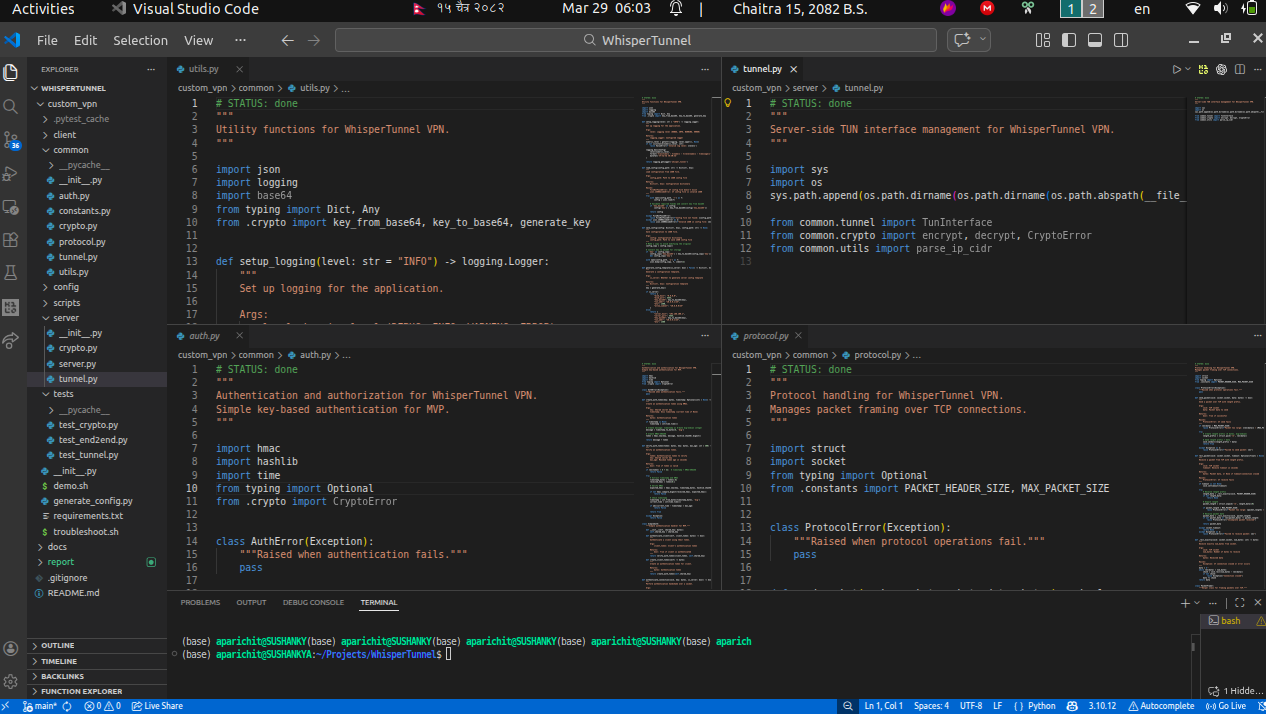
\includegraphics[width=0.95\textwidth]{figures/codebase-shapshot.png}
\caption{Codebase Snapshot}
\label{fig:codebase-snapshot}
\end{figure}

\section{Module Decomposition}
Inside \texttt{custom\_vpn/}, responsibility is layered into shared primitives and endpoint-specific orchestrators.

\subsection{Shared Layer: \texttt{common/}}
\begin{itemize}[leftmargin=2em]
\item \texttt{crypto.py}: AES-GCM encryption/decryption and key conversion.
\item \texttt{protocol.py}: TCP framing and exact-byte receive logic.
\item \texttt{auth.py}: timestamped HMAC token generation and verification.
\item \texttt{tunnel.py}: TUN lifecycle, non-blocking packet I/O, IP configuration.
\item \texttt{utils.py}: config loading/saving, logging, statistics.
\item \texttt{constants.py}: protocol and cryptographic constants.
\end{itemize}

\subsection{Endpoint Layer}
\begin{itemize}[leftmargin=2em]
\item \texttt{client/client.py}: connect/authenticate/setup and bidirectional forwarding.
\item \texttt{server/server.py}: listen/accept/authenticate and forwarding threads.
\end{itemize}

Thin wrappers in \texttt{client/crypto.py}, \texttt{server/crypto.py}, \texttt{client/tunnel.py}, and \texttt{server/tunnel.py} re-export shared functionality and likely exist for organization consistency.

\section{Control Plane and Data Plane Separation}
Code structure naturally separates control actions from packet actions:

\begin{itemize}[leftmargin=2em]
\item \textbf{Control plane}: startup, socket establishment, authentication handshake, thread creation, shutdown handling.
\item \textbf{Data plane}: repeating loops that move packets between TUN and socket with crypto transformations.
\end{itemize}

This split is useful for extension work, because future protocol evolution can be isolated largely to control-plane code while preserving packet loop primitives.

\section{Script Ecosystem}
Operational scripts under \texttt{scripts/} are a major part of usability:

\begin{itemize}[leftmargin=2em]
\item \texttt{netns\_setup.sh}: creates dual namespace topology for local emulation.
\item \texttt{netns\_setup\_internet.sh}: alternative setup with server on host.
\item \texttt{server\_nat.sh}: configures NAT and forwarding rules.
\item \texttt{diagnose.sh}: diagnostics checklist for interfaces/routes/DNS/NAT.
\item \texttt{fix\_internet.sh}: convenience recovery workflow.
\item \texttt{routing.sh}: route rewrite helper.
\end{itemize}

\section{Testing Assets}
The \texttt{tests/} package includes:
\begin{itemize}[leftmargin=2em]
\item Cryptographic behavior tests (round-trip, tamper detection, key validation).
\item TUN interface tests, guarded for root and \texttt{/dev/net/tun} availability.
\item Integration-oriented tests for framing and socket communication.
\end{itemize}

This creates a layered confidence model: pure functions can be validated quickly, while privileged/network tests are opt-in by environment.

\section{Configuration Model}
Configuration is JSON-driven. Client and server files share the same key material using base64 representation:
\begin{itemize}[leftmargin=2em]
\item \texttt{config/client.json}: server endpoint, key, local tunnel address.
\item \texttt{config/server.json}: bind endpoint, key, server tunnel address, allowed subnet hint.
\end{itemize}

The generator script \texttt{generate\_config.py} ensures synchronized key creation for both sides.

\section{Dependency Footprint}
Dependencies are intentionally narrow:
\begin{itemize}[leftmargin=2em]
\item \texttt{cryptography} for AES-GCM operations.
\item \texttt{pyroute2} listed as dependency (not heavily exercised in current code).
\item \texttt{pytest} for test execution.
\end{itemize}

Small dependency surfaces reduce setup complexity for educational use.

\section{Observed Inconsistencies Worth Tracking}
Static inspection reveals a few script-level consistency risks:
\begin{itemize}[leftmargin=2em]
\item Some scripts include Unicode glyphs in output and mixed assumptions about where server runs.
\item \texttt{server\_nat.sh} references \texttt{\$CLIENT\_NS} without local declaration in the visible snippet.
\item Cleanup argument handling in some scripts appears after setup calls, which can cause unintended setup before cleanup.
\end{itemize}

These observations are discussed in risk chapters as operational reliability concerns rather than core protocol flaws.

\section{Summary}
The codebase is compact, understandable, and well suited for educational dissection. Its modular split across \texttt{common/}, endpoint orchestrators, and scripts creates a clear narrative arc for architecture and implementation analysis in the following chapters.

\chapter{System Architecture}

\section{Architectural View}
WhisperTunnel can be represented as two symmetric endpoint stacks connected by a single authenticated TCP channel. Each endpoint stack has three local layers:

\begin{enumerate}[leftmargin=2em]
\item Interface layer: Linux TUN device receives or emits IP packets.
\item Processing layer: encryption/decryption and framing logic.
\item Transport layer: TCP socket handling and thread-managed I/O.
\end{enumerate}

\begin{figure}[H]
\centering
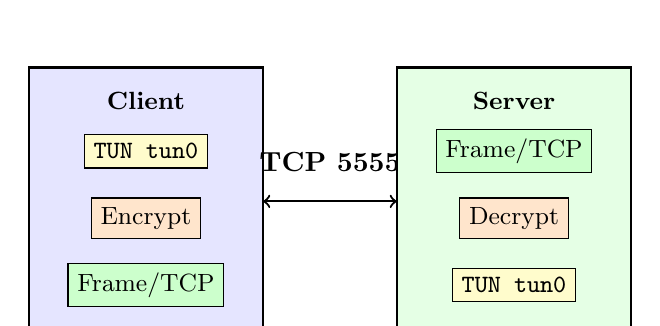
\begin{tikzpicture}[scale=0.85, every node/.style={font=\small}]
  % Client side
  \draw[thick, fill=blue!10] (0,3) rectangle (3.5,7);
  \node at (1.75,6.5) {\textbf{Client}};
  \node[rectangle, draw, fill=yellow!20, minimum height=0.4cm] at (1.75,5.75) {\texttt{TUN tun0}};
  \node[rectangle, draw, fill=orange!20, minimum height=0.4cm] at (1.75,4.75) {Encrypt};
  \node[rectangle, draw, fill=green!20, minimum height=0.4cm] at (1.75,3.75) {Frame/TCP};
  
  % Transport
  \draw[thick, <->] (3.5,5) -- (5.5,5);
  \node[font=\bfseries, above] at (4.5,5.3) {TCP 5555};
  
  % Server side
  \draw[thick, fill=green!10] (5.5,3) rectangle (9,7);
  \node at (7.25,6.5) {\textbf{Server}};
  \node[rectangle, draw, fill=green!20, minimum height=0.4cm] at (7.25,5.75) {Frame/TCP};
  \node[rectangle, draw, fill=orange!20, minimum height=0.4cm] at (7.25,4.75) {Decrypt};
  \node[rectangle, draw, fill=yellow!20, minimum height=0.4cm] at (7.25,3.75) {\texttt{TUN tun0}};
\end{tikzpicture}
\caption{WhisperTunnel System Architecture}
\end{figure}

\section{Lifecycle Sequence}
\subsection{Client}
\begin{enumerate}[leftmargin=2em]
\item Load config and decode base64 key.
\item Establish TCP connection to server.
\item Perform authentication handshake as client.
\item Create and configure \texttt{tun0}.
\item Start two forwarding threads:
  \begin{itemize}[leftmargin=2em]
  \item TUN to socket (encrypt + send).
  \item Socket to TUN (receive + decrypt + inject).
  \end{itemize}
\item Emit periodic stats and handle shutdown signals.
\end{enumerate}

\subsection{Server}
\begin{enumerate}[leftmargin=2em]
\item Load config and decode key.
\item Create and configure \texttt{tun0}.
\item Bind/listen on configured host and port.
\item Accept one client and authenticate.
\item Start forwarding threads equivalent to client directionality.
\item Emit periodic stats, cleanup on termination.
\end{enumerate}

\section{Component Interaction Table}
\begin{table}[H]
\centering
\caption{Primary Runtime Components and Interactions}
\begin{tabular}{p{0.24\textwidth}p{0.30\textwidth}p{0.34\textwidth}}
\toprule
\textbf{Component} & \textbf{Consumes} & \textbf{Produces} \\
\midrule
\texttt{TunInterface} & Kernel-routed IP packets & User-space packet bytes \\
\texttt{encrypt/decrypt} & Plaintext or ciphertext bytes & Ciphertext or plaintext bytes \\
\texttt{PacketFramer} & Byte payloads & Length-delimited stream messages \\
\texttt{authenticate\_connection} & Socket + shared key & Authenticated session state \\
\texttt{Stats} & Packet sizes and error events & Operational counters \\
\bottomrule
\end{tabular}
\end{table}

\section{Threading and Concurrency Model}
Both endpoint processes use a thread-per-direction model for data forwarding. The loops are intentionally simple:

\begin{itemize}[leftmargin=2em]
\item Blocking/timeout I/O keeps CPU usage reasonable.
\item Exceptions break loops and trigger cleanup via \texttt{stop()}.
\item Shared state is small (\texttt{self.running}, sockets, stats counters).
\end{itemize}

This approach is easy to explain and debug but is not the highest-throughput architecture.

\section{Failure Boundaries}
Failure can occur at several boundaries:
\begin{itemize}[leftmargin=2em]
\item Authentication boundary: invalid token or stale timestamp.
\item Crypto boundary: malformed ciphertext, wrong key, tampering.
\item Tunnel boundary: missing privileges or TUN setup failures.
\item Transport boundary: socket disconnects and framing errors.
\end{itemize}

The code responds by logging and exiting loop context, favoring explicit failure over hidden retry complexity.

\section{Representative Flow Snippet}
\begin{lstlisting}[style=vpnpython,caption={Client data-plane pattern (conceptualized from implementation)}]
while self.running:
    packet = self.tun.read_packet(timeout=1.0)
    if packet is None:
        continue
    encrypted = encrypt(packet, self.key)
    self.framer.send(encrypted)
\end{lstlisting}

The mirrored receive path uses \texttt{self.framer.recv()}, then \texttt{decrypt()}, then \texttt{self.tun.write\_packet()}.

\section{Design Trade-Offs}
\begin{table}[H]
\centering
\caption{Notable Trade-Offs}
\begin{tabular}{p{0.30\textwidth}p{0.26\textwidth}p{0.30\textwidth}}
\toprule
\textbf{Decision} & \textbf{Advantage} & \textbf{Cost} \\
\midrule
TCP transport & Simpler reliability/framing model & Added latency, head-of-line blocking \\
Single-client listen(1) & Reduced complexity & No horizontal user scalability \\
Static shared key & Easy setup and deterministic tests & No per-client identity or rotation \\
Threaded loops & Readable control flow & Limited multicore scaling \\
\bottomrule
\end{tabular}
\end{table}

\section{Architecture Integrity Assessment}
Despite MVP constraints, the architecture is coherent:
\begin{itemize}[leftmargin=2em]
\item Responsibilities are mostly localized by module.
\item Packet path is deterministic and auditable.
\item Security controls align with educational scope declarations.
\item Operational scripts bridge theory and runnable environments.
\end{itemize}

The next chapter examines the protocol and cryptography stack in detail, where most correctness and security properties are anchored.

\chapter{Protocol and Cryptography Design}

\section{Protocol Envelope}
WhisperTunnel transmits encrypted packets over TCP by applying a fixed framing convention:
\begin{itemize}[leftmargin=2em]
\item 4-byte unsigned big-endian payload length.
\item Cipher payload of exactly that length.
\end{itemize}

Receiver logic reads exact byte counts using a helper that loops until complete reception or connection failure. This avoids partial-read ambiguity, a common error in stream protocol implementations.

\section{Packet Size Controls}
\texttt{MAX\_PACKET\_SIZE} is derived from default MTU plus overhead cushion. Sender and receiver both enforce this upper bound. Any packet exceeding this threshold raises a protocol error.

\begin{table}[H]
\centering
\caption{Protocol Constants in Current Implementation}
\begin{tabular}{p{0.42\textwidth}p{0.20\textwidth}p{0.24\textwidth}}
\toprule
\textbf{Constant} & \textbf{Value} & \textbf{Meaning} \\
\midrule
\texttt{PACKET\_HEADER\_SIZE} & 4 bytes & Framing length prefix size \\
\texttt{DEFAULT\_MTU} & 1400 bytes & Baseline tunnel payload target \\
\texttt{MAX\_PACKET\_SIZE} & 1500 bytes & Framing safety cap \\
\bottomrule
\end{tabular}
\end{table}

\section{AES-GCM Usage}
Encryption is performed by \texttt{cryptography.hazmat.primitives.ciphers.aead.AESGCM}. For each plaintext packet:
\begin{enumerate}[leftmargin=2em]
\item Validate 32-byte key length.
\item Generate 12-byte random nonce via \texttt{os.urandom}.
\item Encrypt with \texttt{AAD=None}.
\item Emit \texttt{nonce || ciphertext\_with\_tag}.
\end{enumerate}

On decrypt:
\begin{enumerate}[leftmargin=2em]
\item Validate key length.
\item Ensure ciphertext length is at least nonce size.
\item Split nonce and encrypted segment.
\item Attempt decrypt; reject on any authenticity failure.
\end{enumerate}

\section{Why This Is Cryptographically Sound for MVP}
Within its scope, this design avoids several severe beginner pitfalls:
\begin{itemize}[leftmargin=2em]
\item Nonce reuse is unlikely due to cryptographic randomness.
\item Integrity checking is mandatory in GCM decrypt call.
\item Wrong-key and tampering scenarios fail safely through exceptions.
\item Tests explicitly validate tamper detection.
\end{itemize}

\section{Authentication Handshake}
Authentication occurs before packet forwarding begins. The model is symmetric but role-specific:
\begin{itemize}[leftmargin=2em]
\item Client sends token to server.
\item Server validates token and timestamp freshness.
\item Server returns acknowledgment token.
\item Client validates acknowledgment similarly.
\end{itemize}

Token format:
\[
\text{token} = \text{timestamp}_{8\,bytes} || \text{HMAC-SHA256}(key, timestamp)
\]

\begin{figure}[H]
\centering
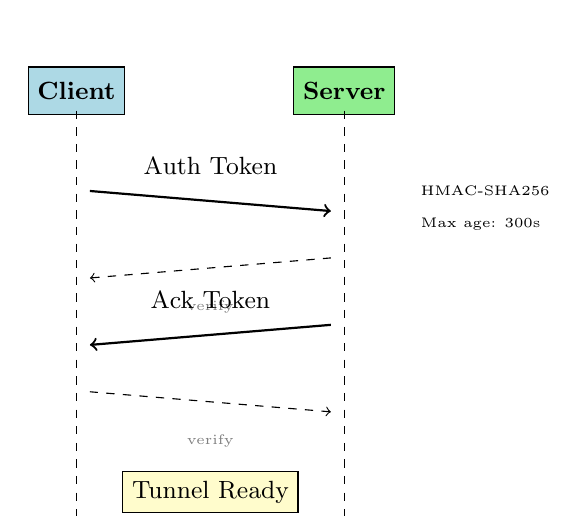
\begin{tikzpicture}[scale=0.85, every node/.style={font=\small}]
  % Actors
  \node[draw, fill=lightblue, minimum height=0.6cm] at (1,7) {\textbf{Client}};
  \node[draw, fill=lightgreen, minimum height=0.6cm] at (5,7) {\textbf{Server}};
  
  % Lifelines
  \draw[dashed] (1,6.7) -- (1,0.5);
  \draw[dashed] (5,6.7) -- (5,0.5);
  
  % 1. Auth Token
  \draw[->, thick] (1.2,5.5) -- (4.8,5.2);
  \node[above, font=\small] at (3,5.6) {Auth Token};
  
  % 2. HMAC Verify
  \draw[<-, dashed] (1.2,4.2) -- (4.8,4.5);
  \node[below, font=\tiny, gray] at (3,4.0) {verify};
  
  % 3. Ack Token
  \draw[->, thick] (4.8,3.5) -- (1.2,3.2);
  \node[above, font=\small] at (3,3.6) {Ack Token};
  
  % 4. Ack Verify
  \draw[<-, dashed] (4.8,2.2) -- (1.2,2.5);
  \node[below, font=\tiny, gray] at (3,2.0) {verify};
  
  % Result
  \node[draw, fill=yellow!20, minimum width=2cm] at (3,1) {Tunnel Ready};
  \node[anchor=west, font=\tiny] at (6,5.5) {HMAC-SHA256};
  \node[anchor=west, font=\tiny] at (6,5.0) {Max age: 300s};
\end{tikzpicture}
\caption{Authentication Handshake Sequence}
\end{figure}

\section{Security Properties and Gaps}
\subsection{Properties Achieved}
\begin{itemize}[leftmargin=2em]
\item Confidentiality for tunnel payload.
\item Per-packet integrity/authenticity at ciphertext level.
\item Basic endpoint possession proof through shared key token exchange.
\end{itemize}

\subsection{Properties Missing}
\begin{itemize}[leftmargin=2em]
\item Perfect forward secrecy.
\item Replay tracking based on sequence state.
\item Distinct key separation for auth and encryption contexts.
\item Negotiated protocol versioning and cipher agility.
\end{itemize}

\section{Replay Discussion}
Timestamp-limited tokens constrain stale authentication messages but do not prevent replay of encrypted data packets in-session because packet-level sequence windows are absent. Random nonces protect GCM uniqueness but are not replay identifiers in this protocol.

\section{Code Listing: Framing Primitive}
\begin{lstlisting}[style=vpnpython,caption={Length-prefix send pattern from protocol module}]
def send_packet(sock, data):
    if len(data) > MAX_PACKET_SIZE:
        raise ProtocolError("Packet too large")
    length_prefix = struct.pack('>I', len(data))
    sock.sendall(length_prefix + data)
\end{lstlisting}

\section{Code Listing: Auth Token Generation}
\begin{lstlisting}[style=vpnpython,caption={Timestamped HMAC token generation pattern}]
def create_auth_token(key, timestamp=None):
    if timestamp is None:
        timestamp = int(time.time())
    message = timestamp.to_bytes(8, 'big')
    token = hmac.new(key, message, hashlib.sha256).digest()
    return message + token
\end{lstlisting}

\section{Protocol Hardening Recommendations}
Short-term upgrades that preserve educational readability:
\begin{enumerate}[leftmargin=2em]
\item Add packet sequence counters and replay window tracking.
\item Split secrets into dedicated subkeys via HKDF.
\item Include protocol version and flags in a small fixed header.
\item Bind metadata into AEAD AAD to prevent cross-context misuse.
\item Define explicit error codes for auth/protocol failures.
\end{enumerate}

\section{Conclusion}
The protocol and crypto stack is coherent and appropriately small for teaching. It correctly demonstrates modern AEAD usage and stream framing, while leaving clear room for advanced defensive mechanisms in future iterations.

\chapter{Implementation Walkthrough}

\section{Client Implementation Path}
The \texttt{VPNClient} class orchestrates startup and forwarding. Constructor logic validates required config keys, initializes endpoint parameters, and prepares runtime state containers (socket, framer, tun interface, threads, stats).

\subsection{Startup Sequence}
The operational sequence in \texttt{start()} is clear and linear:
\begin{enumerate}[leftmargin=2em]
\item Register signal handlers for graceful shutdown.
\item Connect to server over TCP.
\item Authenticate via \texttt{authenticate\_connection(..., is\_server=False)}.
\item Initialize \texttt{PacketFramer} over connected socket.
\item Set up TUN interface and assign configured tunnel IP.
\item Start two forwarding threads.
\item Enter periodic stats loop until termination.
\end{enumerate}

\section{Server Implementation Path}
\texttt{VPNServer} mirrors client logic but adds passive listen/accept behavior. Notable server-specific details:
\begin{itemize}[leftmargin=2em]
\item Socket configured with \texttt{SO\_REUSEADDR}.
\item \texttt{listen(1)} enforces single client in MVP.
\item Accept thread performs auth before starting packet forwarding.
\end{itemize}

\section{TUN Interface Abstraction}
\texttt{TunInterface} encapsulates Linux-specific setup:
\begin{itemize}[leftmargin=2em]
\item \texttt{/dev/net/tun} is opened with read/write flags.
\item \texttt{ioctl(TUNSETIFF)} creates configured TUN device.
\item File descriptor is switched to non-blocking mode.
\item Interface IP and MTU are configured through \texttt{ip} commands.
\end{itemize}

Packet reads use \texttt{select.select} with timeout, enabling loops to stay responsive to \texttt{self.running} changes.

\section{Utilities and Shared Services}
\subsection{Config Pipeline}
\texttt{load\_config()} reads JSON and automatically decodes \texttt{key\_base64} into raw bytes for runtime crypto calls. This keeps endpoint code uncluttered and prevents repetitive decoding logic.

\subsection{Statistics}
\texttt{Stats} tracks packet and byte counters for each direction plus decrypt failures. The string representation is log-friendly and suitable for periodic heartbeat diagnostics.

\section{Error Handling Philosophy}
Implementation favors explicit exception capture by category:
\begin{itemize}[leftmargin=2em]
\item Tunnel failures raise \texttt{TunnelError}.
\item Framing/socket issues raise \texttt{ProtocolError} or socket exceptions.
\item Crypto faults raise \texttt{CryptoError} and increment failure counters.
\end{itemize}

This approach is understandable for learners because failure sources remain visible in logs and map directly to subsystem boundaries.

\section{Code Listing: Receive-Decryption-Inject Loop}
\begin{lstlisting}[style=vpnpython,caption={Data-plane receive path pattern from client/server loops}]
encrypted_packet = self.framer.recv(timeout=1.0)
if encrypted_packet is None:
    continue
packet = decrypt(encrypted_packet, self.key)
self.tun.write_packet(packet)
self.stats.record_packet_in(len(packet))
\end{lstlisting}

\section{Scripted Environment Workflows}
Implementation is supported by shell utilities to reduce manual setup burden. Scripts create namespaces, veth links, forwarding rules, DNS files, and cleanup paths. This ecosystem effectively functions as a deployment harness for demonstrations.

\begin{figure}[H]
\centering
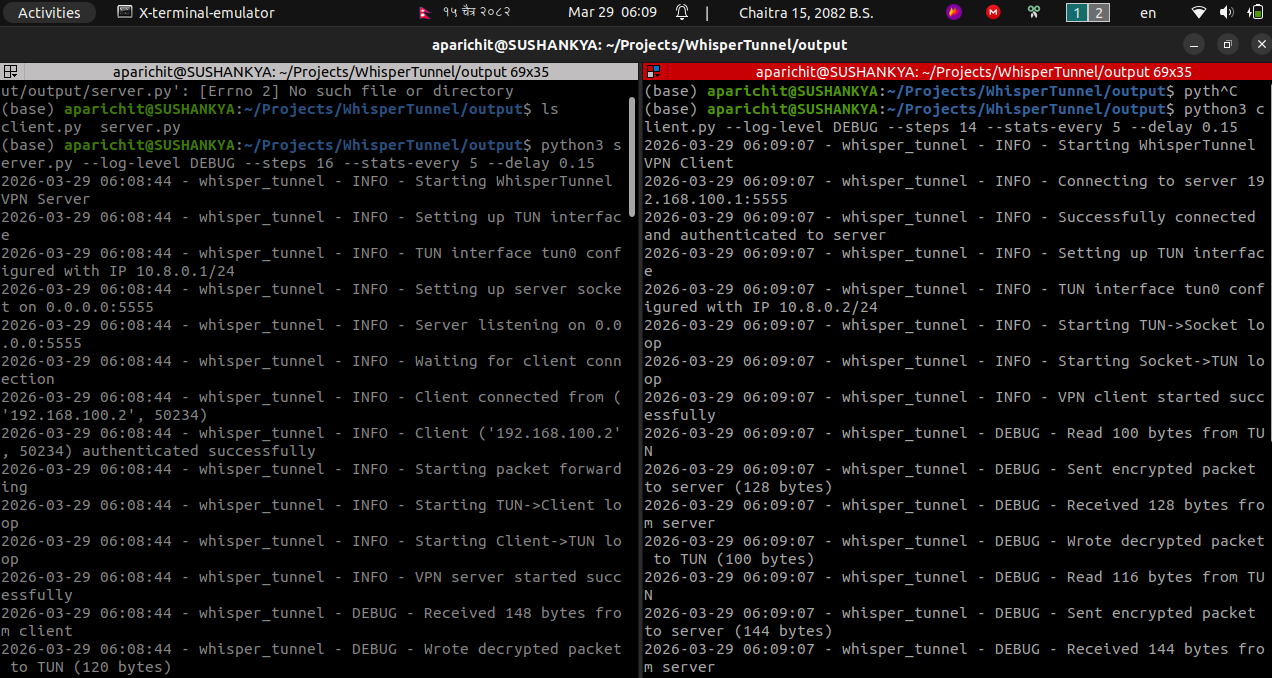
\includegraphics[width=0.95\textwidth]{figures/runtime-shapshot.png}
\caption{Runtime Snapshot of Server and Client Logs}
\label{fig:runtime-snapshot}
\end{figure}

\section{Potential Refactors for Maintainability}
Several clean refactors can improve maintainability without changing functionality:
\begin{enumerate}[leftmargin=2em]
\item Extract shared loop logic into a generic forwarding worker.
\item Add structured lifecycle state machine to reduce flag-based control.
\item Introduce dataclass-based config models with typed validation.
\item Normalize script variables and strict shell linting.
\item Replace duplicate wrapper modules with explicit import conventions.
\end{enumerate}

\section{Complexity Profile}
The implementation remains compact, with most technical complexity concentrated in three files:
\begin{itemize}[leftmargin=2em]
\item \texttt{client/client.py}
\item \texttt{server/server.py}
\item \texttt{common/tunnel.py}
\end{itemize}

This concentration is favorable for educational walkthroughs because students can understand end-to-end behavior by mastering a small subset of files.

\section{Observations on Operational Robustness}
While code pathways are clear, robustness constraints include:
\begin{itemize}[leftmargin=2em]
\item Limited reconnection behavior.
\item No backoff strategy for transient network issues.
\item Single-client server assumptions in socket acceptance.
\item Script-level variance in namespace and host execution expectations.
\end{itemize}

These constraints are expected for MVP educational systems and become roadmap candidates rather than immediate defects.

\chapter{Deployment and Operations}

\section{Execution Models}
The repository supports two practical execution models:
\begin{enumerate}[leftmargin=2em]
\item \textbf{Dual-namespace model}: both server and client run in separate namespaces.
\item \textbf{Host-server model}: server runs on host, client runs in namespace (for easier internet NAT).
\end{enumerate}

Scripts suggest both models are used for different troubleshooting and internet-access scenarios.

\section{Baseline Setup Procedure}
A canonical setup path from repository assets:
\begin{enumerate}[leftmargin=2em]
\item Install Python dependencies via \texttt{pip install -r requirements.txt}.
\item Generate synchronized client/server configs via \texttt{generate\_config.py}.
\item Initialize namespaces via \texttt{scripts/netns\_setup.sh}.
\item Start server then client in target execution contexts.
\item Validate tunnel reachability with ping to \texttt{10.8.0.1}.
\end{enumerate}

\section{Operational Runbook Table}
\begin{table}[H]
\centering
\caption{Operational Commands and Purpose}
\begin{tabular}{p{0.42\textwidth}p{0.44\textwidth}}
\toprule
\textbf{Command Pattern} & \textbf{Purpose} \\
\midrule
\texttt{python3 generate\_config.py} & Create fresh synchronized configs \\
\texttt{sudo bash scripts/netns\_setup.sh} & Build client/server namespace topology \\
\texttt{sudo ip netns exec vpn-server ...server.py} & Start server in namespace \\
\texttt{sudo ip netns exec vpn-client ...client.py} & Start client in namespace \\
\texttt{sudo bash scripts/server\_nat.sh} & Configure NAT and forwarding \\
\texttt{sudo bash scripts/diagnose.sh} & Automated diagnostics for connectivity \\
\bottomrule
\end{tabular}
\end{table}

\section{NAT and Internet Access Path}
Internet access from the VPN client is achieved through host NAT rules. The script configures:
\begin{itemize}[leftmargin=2em]
\item \texttt{net.ipv4.ip\_forward=1}
\item \texttt{iptables -t nat POSTROUTING MASQUERADE}
\item FORWARD rules between tunnel and host egress interface
\item Namespace DNS configuration under \texttt{/etc/netns/vpn-client/resolv.conf}
\end{itemize}

\begin{figure}[H]
\centering
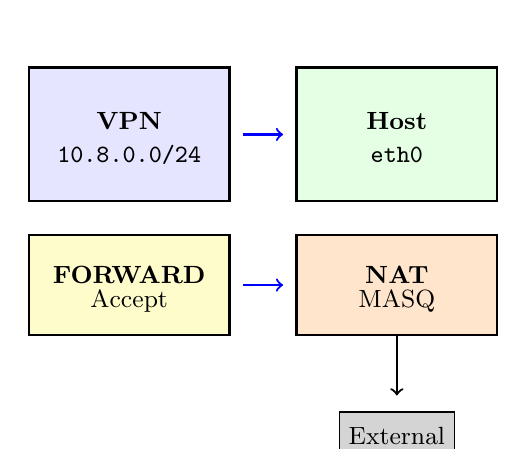
\begin{tikzpicture}[scale=0.85, every node/.style={font=\small}]
  % VPN Subnet
  \draw[thick, fill=blue!10] (0.5,5) rectangle (3.5,7);
  \node at (2,6.2) {\textbf{VPN}};
  \node at (2,5.7) {\texttt{10.8.0.0/24}};
  
  % Iptables FORWARD
  \draw[thick, fill=yellow!20] (0.5,3) rectangle (3.5,4.5);
  \node at (2,3.9) {\textbf{FORWARD}};
  \node at (2,3.5) {\small Accept};
  
  % NAT POSTROUTING
  \draw[thick, fill=orange!20] (4.5,3) rectangle (7.5,4.5);
  \node at (6,3.9) {\textbf{NAT}};
  \node at (6,3.5) {\small MASQ};
  
  % Host Interface
  \draw[thick, fill=green!10] (4.5,5) rectangle (7.5,7);
  \node at (6,6.2) {\textbf{Host}};
  \node at (6,5.7) {\texttt{eth0}};
  
  % Flow arrows
  \draw[->, thick, blue] (3.7,6) -- (4.3,6);
  \draw[->, thick, blue] (3.7,3.75) -- (4.3,3.75);
  
  % Destination
  \node[draw, fill=lightgray, minimum height=0.6cm] at (6,1.5) {External};
  \draw[->, thick] (6,3) -- (6,2.1);
\end{tikzpicture}
\caption{NAT and Forwarding Configuration}
\end{figure}

\section{Diagnostics Workflow}
\texttt{scripts/diagnose.sh} provides a useful fault-isolation checklist:
\begin{enumerate}[leftmargin=2em]
\item Verify namespaces exist.
\item Verify \texttt{tun0} presence and address.
\item Test tunnel ping.
\item Inspect routes and DNS configuration.
\item Check forwarding and NAT rules.
\item Test external reachability and optional HTTP response.
\end{enumerate}

This script-driven checklist lowers debugging time and creates a reproducible support process.

\section{Operational Risks Observed in Scripts}
From static review, operations scripts include a few consistency risks:
\begin{itemize}[leftmargin=2em]
\item Variable scope assumptions in NAT script (client namespace variable reference).
\item Cleanup argument handling appears near script tail in some files.
\item Mixed assumptions about server location (host vs namespace) across helper scripts.
\end{itemize}

These are manageable but should be normalized to avoid user confusion.

\section{Hardening the Operational Surface}
Recommended improvements:
\begin{enumerate}[leftmargin=2em]
\item Add strict mode in shell scripts: \texttt{set -euo pipefail}.
\item Centralize shared script variables in one sourced file.
\item Make cleanup handlers early and idempotent.
\item Emit explicit mode banner: \texttt{host-server} vs \texttt{dual-namespace}.
\item Add script tests in CI using containerized Linux testbeds.
\end{enumerate}

\section{Observability}
Current observability is log-centric with periodic stats from Python processes. Operational maturity can be improved with:
\begin{itemize}[leftmargin=2em]
\item Structured logging fields (namespace, endpoint role, flow direction).
\item Exportable counters (Prometheus textfile, JSON snapshots).
\item Optional packet trace mode for controlled debugging.
\end{itemize}

\section{Deployment Profiles}
\begin{table}[H]
\centering
\caption{Suggested Deployment Profiles}
\begin{tabular}{p{0.27\textwidth}p{0.24\textwidth}p{0.35\textwidth}}
\toprule
\textbf{Profile} & \textbf{Primary Goal} & \textbf{Recommended Settings} \\
\midrule
Learning lab & Concept demonstration & Dual namespace, verbose logs, debug scripts \\
Classroom demo & Reliable reproducibility & Host-server mode, prebuilt configs, scripted launch \\
Research prototype & Extend architecture & Add packet IDs, benchmark hooks, profile tooling \\
\bottomrule
\end{tabular}
\end{table}

\section{Takeaway}
WhisperTunnel's operational tooling is unusually rich for an educational repository. It already enables realistic demonstrations and debugging workflows, and with script normalization it can provide near turnkey lab reproducibility.

\chapter{Conclusion and Roadmap}

\section{What WhisperTunnel Achieves Well}
WhisperTunnel succeeds as an educational VPN implementation by combining practical realism with readable code. It demonstrates core building blocks that many learners struggle to connect in one coherent system:
\begin{itemize}[leftmargin=2em]
\item TUN-driven packet interception and injection.
\item Authenticated encryption of packet payloads.
\item Stream-safe packet framing over TCP.
\item Namespace-based deployment and validation workflows.
\item Scripted operations and diagnostics.
\end{itemize}

\section{Most Important Findings from Codebase Study}
\begin{enumerate}[leftmargin=2em]
\item Architecture is modular and conceptually clean.
\item Crypto usage is generally correct for MVP educational scope.
\item Testing is meaningful and better than typical small prototypes.
\item Operational scripts provide strong demonstrability but need consistency cleanup.
\item Security and scalability gaps are explicit and tractable.
\end{enumerate}

\section{Roadmap by Milestones}
\subsection{Milestone 1: Protocol Safety Upgrade}
\begin{itemize}[leftmargin=2em]
\item Add packet sequence numbers and anti-replay window.
\item Add protocol version field and capability negotiation.
\item Separate auth/encryption keys through KDF.
\end{itemize}

\subsection{Milestone 2: Session Security Upgrade}
\begin{itemize}[leftmargin=2em]
\item Introduce ephemeral key exchange for forward secrecy.
\item Implement periodic rekey and key lifetime limits.
\item Add explicit session teardown messages.
\end{itemize}

\subsection{Milestone 3: Scale and Resilience Upgrade}
\begin{itemize}[leftmargin=2em]
\item Multi-client server state management.
\item Reconnection and backoff strategy.
\item Optional UDP transport profile.
\end{itemize}

\subsection{Milestone 4: Productization Foundations}
\begin{itemize}[leftmargin=2em]
\item CI pipeline for unit/integration/privileged tests.
\item Packaging, service units, and config validation tooling.
\item Structured observability and release engineering discipline.
\end{itemize}

\section{Educational Impact}
For students and early-career engineers, the project is particularly valuable because it exposes interactions between OS networking, cryptographic APIs, socket protocols, and operations automation. The codebase is compact enough for complete comprehension but rich enough to teach real engineering trade-offs.

\section{Recommended Next Experiments}
\begin{enumerate}[leftmargin=2em]
\item Implement packet sequence IDs and measure replay rejection behavior.
\item Prototype UDP transport with controlled loss tests.
\item Compare namespace-only versus host-server deployment reliability.
\item Add benchmark harness and publish reproducible performance tables.
\item Write threat-driven tests for malformed framing and auth abuse.
\end{enumerate}

\section{Final Statement}
WhisperTunnel is already a strong teaching artifact and a credible base for incremental research-grade enhancements. With targeted security hardening and performance instrumentation, it can evolve from educational MVP to a robust experimental VPN platform while preserving the clarity that makes it valuable.


\backmatter

\chapter*{Bibliographic Notes}
This report references implementation facts from the WhisperTunnel codebase and its embedded documentation, especially \texttt{README.md} and \texttt{docs/design.md}. Conceptual framing is informed by standard VPN and AEAD literature, including AES-GCM usage practices and Linux namespace/TUN workflows.

\end{document}
